%-----------------------------------------------------------------------
%\subsection{Proof of concept}
%-----------------------------------------------------------------------
%\tbc
%Baseliyos Jacob and Jakob G.

\section{Proof of concept on the Track Utrecht Amsterdam User Stories 1 - 4}

The goal of the openETCS@ITEA2 project is to deliver at the and a proof of concept in a lab on a real ETCS Track. Since the Level 2 Utrecht - Amsterdam track was evaluated as the most approriate reference track for this concept due the maturity and representative of the track, it will be use for the mentioned simulation.\\

To start with the realisation of the concept in a iterative way in the same pattern the industry is proceeding and an regarding the "classical" state of the art of sytemanalisiys we started in this third iteration with the following Use Cases and Scenarios:\\

\subsection{Use Case and Scenario 1}
\textbf{Start of Mission - Awakening of the Train:}
This use case according to the procedure in chapter 5 will demonstrate the start of a train from a no power modus to the state that train will be ready for level and mode change according to the chapter 5.\\ 
Link on Git-Hub \url{https://github.com/openETCS/modeling/issues/66}

The following Subsystems needs to be realised for Scenario 1:\\
\begin{itemize}
\item Procedure
\item TIU Management
\item DMI Management and Controller
\item Position Report
\item Management of Radio Communication
\item Manage Track Data
\item Manage Mode and Level
\item Train Supervision
\end{itemize}

\subsection{Use Case and Scenario 2}
\textbf{Start of Mission - Start in Level 2 Mode FS:}
This use case according to the procedure in chapter 5 will demonstrate the start of a train from the awakening of the train in mode stand by to the state that train will receive a movement authority in level 2 and change into the mode full supervision to start running under real supervision according to the chapter 5.\\ 
link on Git-Hub \url{https://github.com/openETCS/modeling/issues/67}

The following Subsystems needs to be realised for Scenario 2:\\
\begin{itemize}
\item Procedure
\item TIU Management
\item DMI Management and Controller
\item Position Report
\item Management of Radio Communication
\item Manage Track Data
\item Manage Mode and Level
\item Train Supervision
\end{itemize}

\subsection{Use Case and Scenario 3}
\textbf{Brake intervention - Revocation of a Movement Authority and Overrun Permitted Speed:}
This use case according to the subset 26 chapter 3 principles will demonstrate the brake intervention that will cause by a revocation of a movement authority due to a occupied section or track an due simple overrun of a permitted speed  according to the chapter 3.\\ 
Link on Git-Hub \url{https://github.com/openETCS/modeling/issues/68}

The following Subsystems needs to be realised for Scenario 3:\\
\begin{itemize}
\item Procedure
\item TIU Management
\item DMI Management and Controller
\item Position Report
\item Management of Radio Communication
\item Manage Track Data
\item Manage Mode and Level
\item Train Supervision
\end{itemize}

\subsection{Use Case and Scenario 4}
\textbf{ETCS Onboard Unit is reading and sending track information:}
This use case according to the subset 26 chapter 3 principles will demonstrate the full completeness and checking the reading and sending of track information in interaction with the ETCS Onboard Unit and the track that will be separated in radio and balise messages. Messages and packages are defined in chapter 7 and 8 of the subset 26.\\ 
Link on Git-Hub \url{https://github.com/openETCS/modeling/issues/69}

The following Subsystems needs to be realised for Scenario 4:\\
\begin{itemize}
\item Procedure
\item TIU Management
\item DMI Management and Controller
\item Position Report
\item Management of Radio Communication
\item Manage Track Data
\item Manage Mode and Level
\item Train Supervision
\item Building of coordinate system
\end{itemize}

%\tbc
%Jakob G.
\section{Environment model for the use case demonstrations}

%
% 
%
%


In order to dynamically explore and demonstrate the openETCS OBU kernel software, a dynamic simulation and demonstration environmental model is being created.
During Iteration 3, this comprises the following features and functionalities:\\
•   openETCS OBU formal model \\
•   openETCS DMI formal model with Display specification model\\
•      Simplified version, not all features are implemented yet; following our use- case driven approach we are only implementing features that are essential to show the use cases selected by our "internal customer".\\
•    Environment model with \\
•  	- simplified track model (balise locations, speed profile)\\
•  	- simplified model of Movement Authority\\
•  	- interactive widgets to manipulate the simulation environment\\
\\
\\
\\

%\tbc
%Jakob G.
(see Figure \ref{fig:WP3-demo}.)
	
\begin{figure}
  \centering
  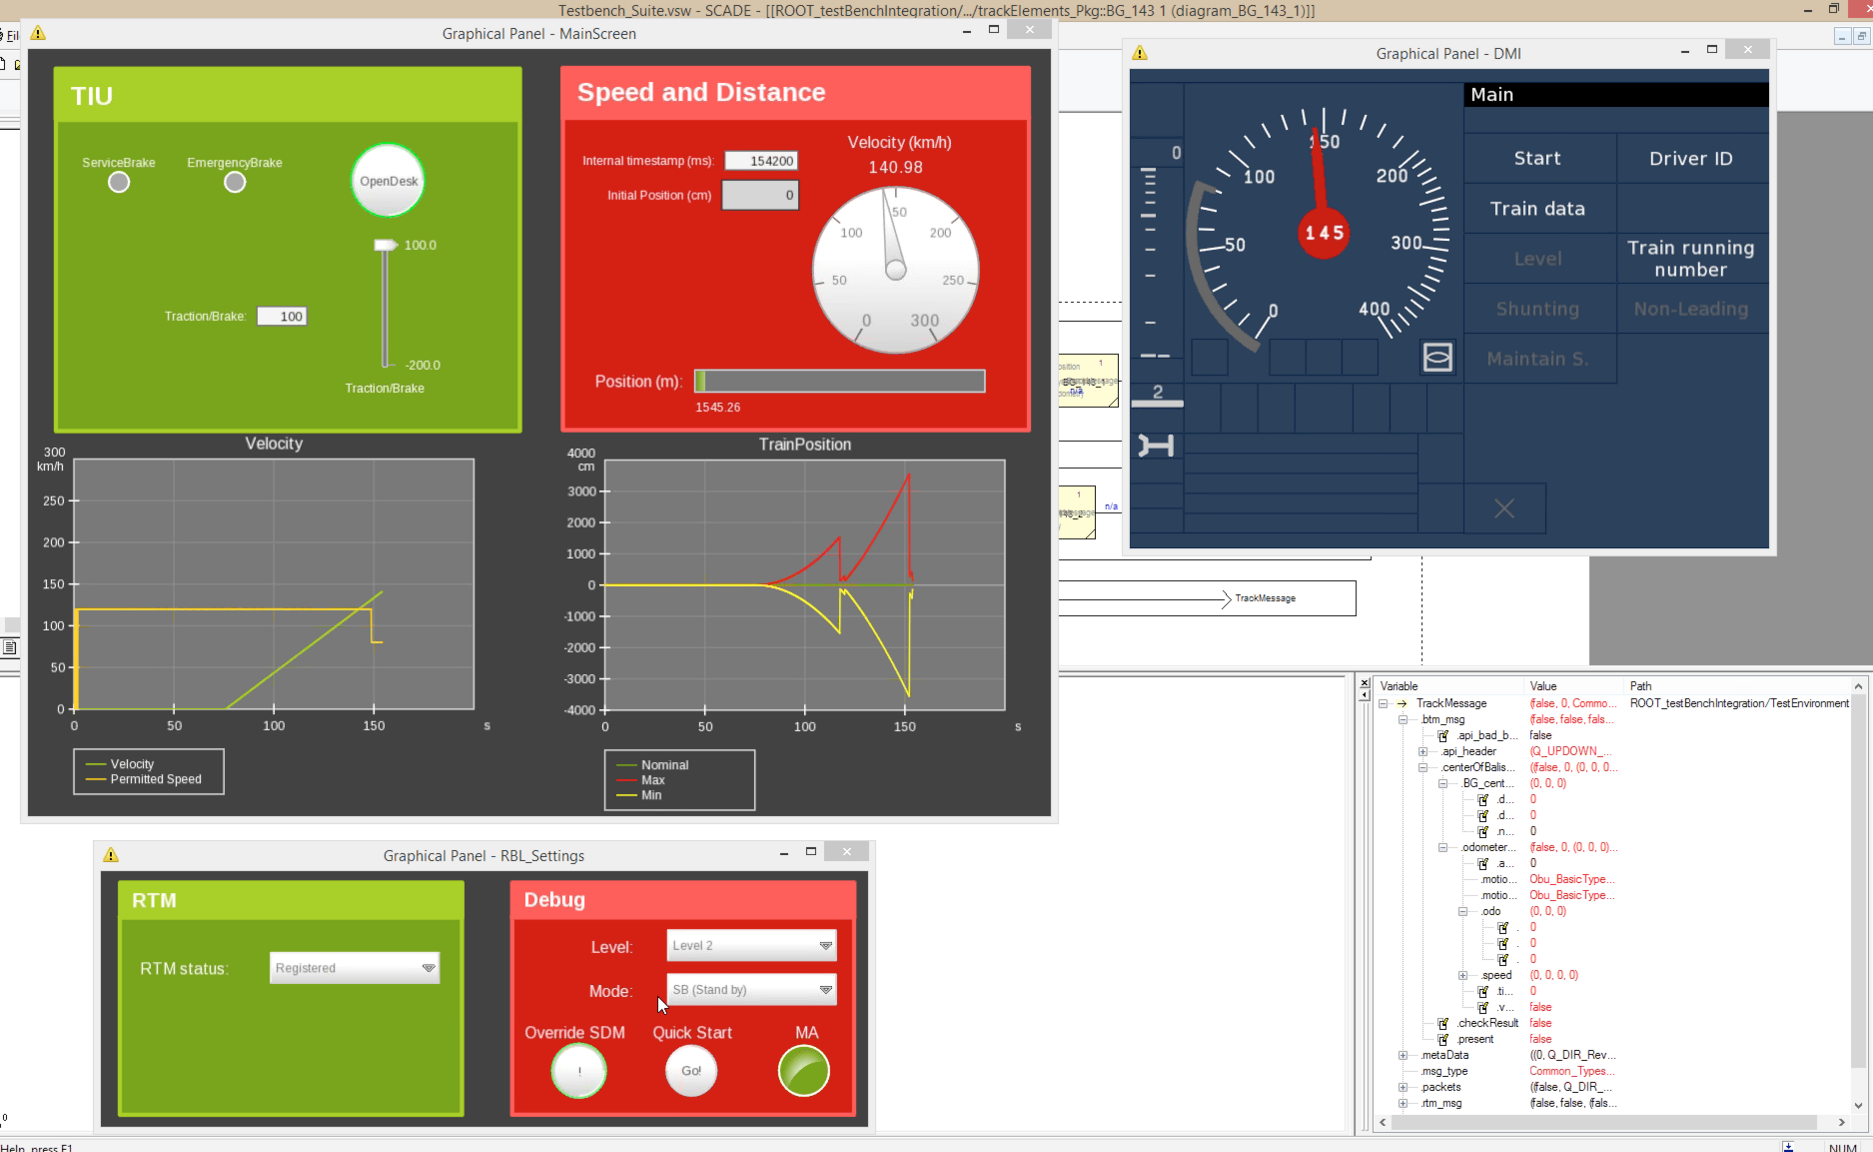
\includegraphics[width=\linewidth]{POC_environment.png}
  \caption{Environment for use case demonstration}
  \label{fig:WP3-demo}
\end{figure}




\section{Dynamic track model of the ETCS Level 2 line Amsterdam- Utrecht}

This environment model will be fourthly enhanced during the last project period, in order to:\\

•   Allow full dynamic simulation of the Utrecht- Amsterdam line\\
•   Form a basis for a (future) dynamic track simulator, which models the balise locations, balise messages and RBC messages for any given line, and which can automatically be generated from engineering datasets.\\
•   Provide a full track model for the purposes of openETCS\\

The principle of this model is shown in Figure \ref{fig:track-dynamic}. 
The idea is to split the model in two parts:\\
•  	Generic functions, that represent the behaviour of the trackside installations (for example balise groups, RBC reception, RBC sending)\\
•  	Data that instantiate these generic functions (for example balise locations, balise message/ packet data, radio message/ packet data)\\

This simulation approach is designed to be adaptable to very different kinds of scenarios:\\

•  	Proof of concept in openETCS: Amsterdam- Utrecht line\\
In that case we have a partially known line (balise locations and track topology are known, messages and packets are known "as-is" from JRU data owned by the partners.
We have been using SCADE graphical notation for the development of the concept in order to disseminate it more easily.
The models will however be instantiated by automatic conversion of engineering and JRU data to simulation scenarios for "nominal" operations validation.
Specific test cases will either be transformed by script from test data bases (in WP4) or can also be graphically modelled (for user validation scenarios or demonstration purposes).\\
•  	OBU validation for existing tracks\\
Once the concept and simulation environment have been validated in openETCS context, the tooling can be used to import track data from other tracks, such as the Corridor A, in order to develop interoperable ETCS specifications. \\
•  	Track validation for existing OBUs (or against the TSI)
With a validated OBU software model, the system can also be used to validate new track layouts.\\
Dynamic track simulation opens new dimensions of attacking the interoperability issues that Europe is facing.\\
%
%
%\tbc
%Jakob G.
\subsection{Model concept}

Traditionally, most ETCS simulators use predefined simulation scenarios, which define the inputs to the model at predefined steps.
They can either be time triggered (update every n time units), distance- oriented (update every n distance units) or cycle- oriented (update every simulation cycle)

The disadvantage of such an approach is clear: all parameters have to be predefined and pre-validated, for example to simply make sure that the time/ distance ratio is consistent.
In such a setting it is very difficult to simulate events in just one dimension (independently of the other parameters).

By creating functional models of the track elements and combining them with data we are now able to explore much more complex scenarios with for example interactive driver interaction, thus not only exploring the implementation of the OBU or the engineering / layout of the track, but also the impact on operational procedures, human factors.

As all events can be recorded and replayed and are based on a formal model (also for the track model and engineering data), the entire environment can be validated and potentially even be certified.
The same EN50128 certifiable toolchain is used that serves the consortium for modelling of the OBU itself.

The basic concept is very simple, but can be developed into a full dynamic track and RBC model.
\begin{figure}
  \centering
  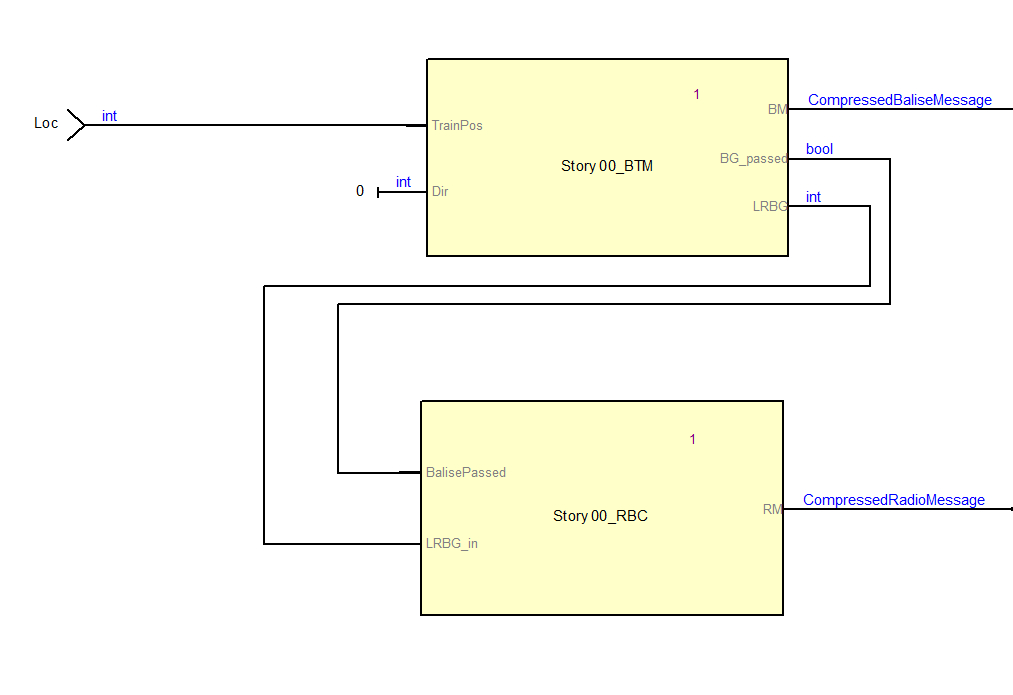
\includegraphics[width=\linewidth]{POC-story00.png}
  \caption{High- level view of dynamic model with Balises and Radio Block Center}
  \label{fig:track-story00}
 \end{figure}
One functional block represents the balises, one functional block represents the RBC (see Figure \ref{fig:track-story00}.) When train movement is simulated, the functional blocks representing the balises and the RBC, respectively, receive the steadily updated train position (via the input "Loc") and react accordingly.
When a balise group detects a passing train, it reacts accordingly by emitting the defined messages and packets.

In an analog way, the RBC block reacts as defined when it receives a train to track message from the simulated OBU by emitting the appropriate set of messages and packets.
While the functionality of the balise groups is modelled in order to reflect their behaviour, they are instantiated using parameter sets that are defined as SCADE constants.
One dataset each defines:\\

•  	Balise positions (from engineering data)\\
(see Figure \ref{fig:Balise-Position-Data}.)\\

In this example, the balise's engineering data have a local coordinate system (km on track, nominal orientation in direction of Amsterdam or Utrecht, respectively, and orientation of the line (Z= zuid, Dutch for southbound, N= northbound)

\begin{figure}
  \centering
  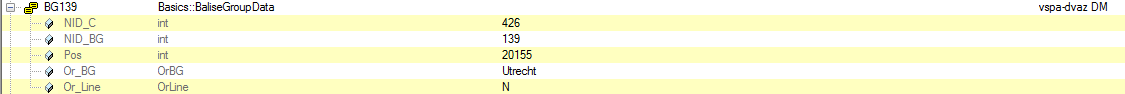
\includegraphics[width=\linewidth]{Balise-Position-Data.png}
  \caption{Example of balise position data}
  \label{fig:Balise-Position-Data}
\end{figure}

•  	Balise messages and packets (from JRU data)\\
(see Figure \ref{fig:BalsieMessageHeaders}.)\\

\begin{figure}
  \centering
  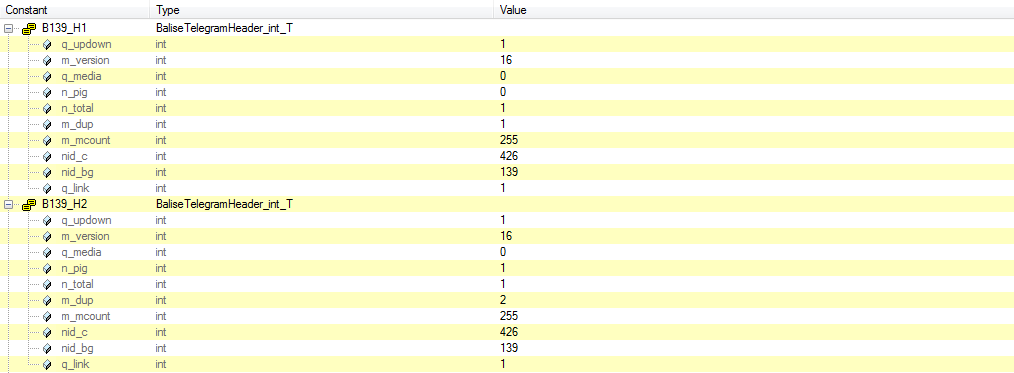
\includegraphics[width=\linewidth]{BalsieMessageHeaders.png}
  \caption{Example of Balise Message Header Data}
  \label{fig:BalsieMessageHeaders}
\end{figure}

Actual data from the Utrecht- Amsterdam line can be seen in this example. Typical for a Level 2 line is that most balise groups are only used as positional reference for the train.
The balise groups are then put together to a "track" which emits telegrams as the train "passes" over it.
This concept is scaleable and the balises can equally instantiated using textual Scade models which can automatically from (for example) JRU data.
(see Figure \ref{fig:Balises5}.)\\
	
\begin{figure}
  \centering
  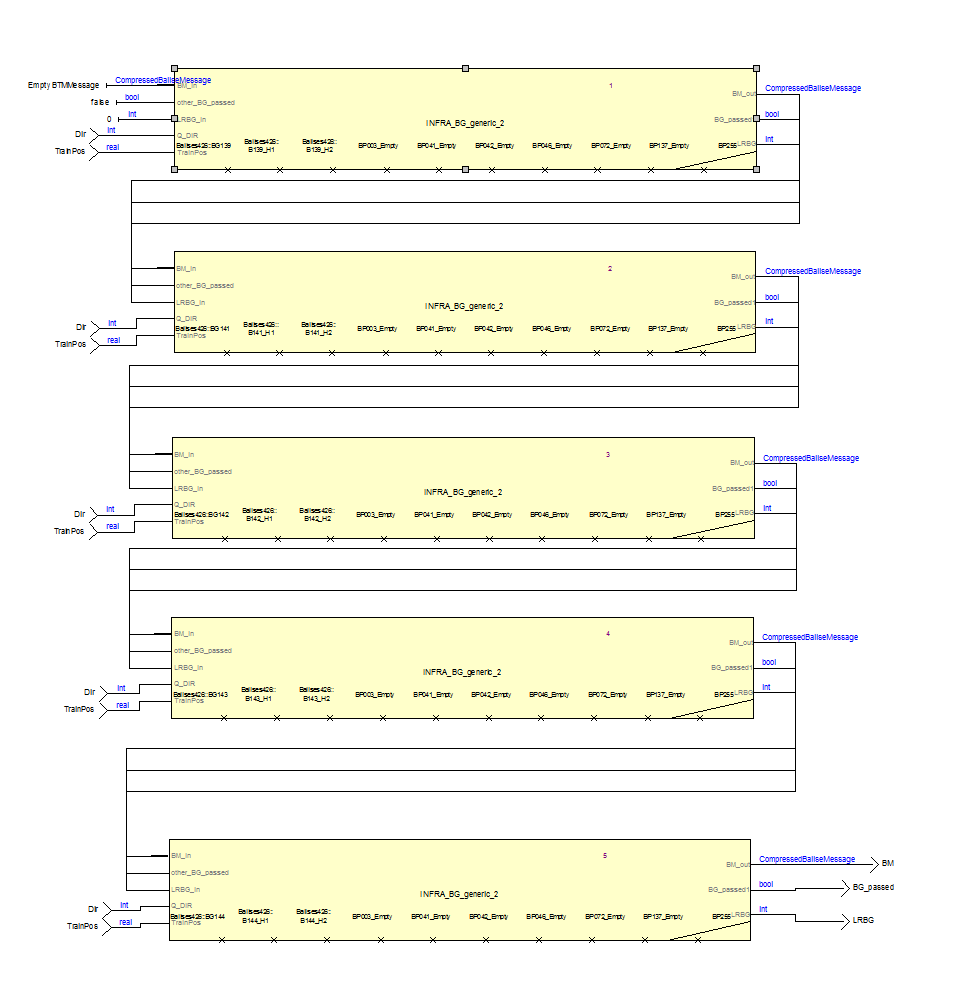
\includegraphics[width=\linewidth]{Balises5.png}
  \caption{Graphical representation of five balise groups}
  \label{fig:Balises5}
\end{figure}

•  	RBC messages and packets (from JRU data). The modelling of the RBC follows a heavily simplified concept at the moment: The simulated RBC emits telegrams/messages/packets in predefined situations. For example, the reception of a specific train-to-track message such as a specific position report triggers emission of a set of messages and packets, such as a complete Movement Authority message with packets for international static speed profile, national values, gradient profile, MA, etc.
The functional block may seamlessly be replaced with a full RBC simulation. \ref{fig:RBC-example-data}. shows a dataset representing RBC packets in SCADE constant format.

\begin{figure}
  \centering
  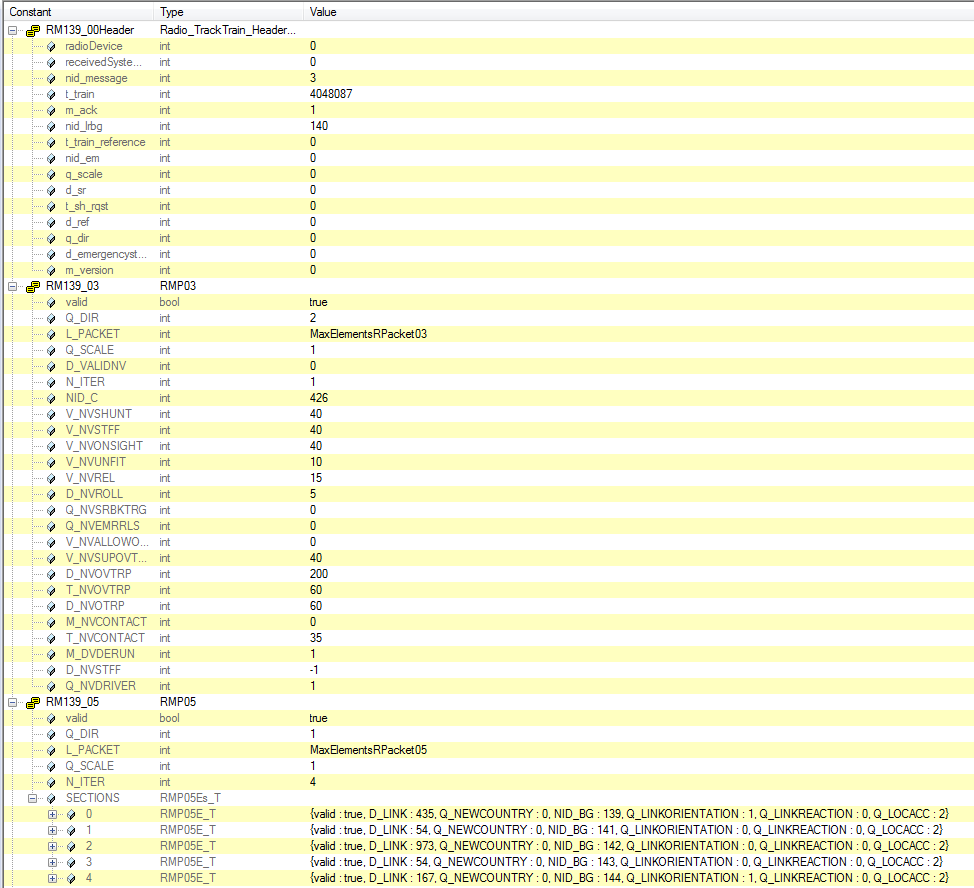
\includegraphics[width=\linewidth]{RBC-example-data.png}
  \caption{Example of Radio Message and Packet data}
  \label{fig:RBC-example-data}
\end{figure}
•  	Potentially, any required data set can be defined on both the input side (static data or scenarios) and on the output side (expected outcome for validation)

%
%
%
%
